%%%%%%%%%%%%%%%%%%%%%%%%%%%%%%%%%%%%%%%%%%%%%%%%%%%%%%%%%%%%%%%%%%%%%%%%%%%
%% This file is part of the book
%%
%% Algorithmic Graph Theory
%% http://code.google.com/p/graph-theory-algorithms-book/
%%
%% Copyright (C) 2009--2011 Minh Van Nguyen <nguyenminh2@gmail.com>
%%
%% See the file COPYING for copying conditions.
%%%%%%%%%%%%%%%%%%%%%%%%%%%%%%%%%%%%%%%%%%%%%%%%%%%%%%%%%%%%%%%%%%%%%%%%%%%

\documentclass{article}

\usepackage{tikz}
\usetikzlibrary{external}
\tikzexternalize{Kruskal-example}

\begin{document}

\begin{figure}
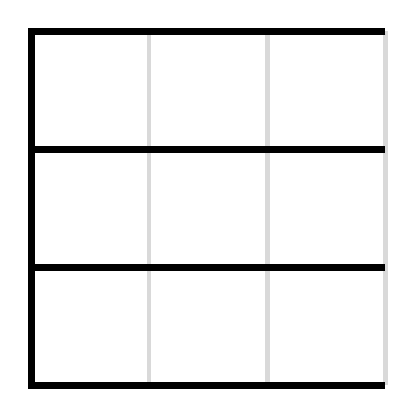
\begin{tikzpicture}
[darkLine/.style={line width=2.5pt},%
  lightLine/.style={-,ultra thick,color=gray!30},%
  scale=1.5]
\foreach \x/\ystart/\yend in {1/0/3, 2/0/3, 3/0/3}
{
  \draw[lightLine] (\x,\ystart) -- (\x,\yend);
}
%% draw the spanning tree
\draw[darkLine] (3,3) -- (0,3) -- (0,0) -- (3,0);
\draw[darkLine] (0,1) -- (3,1);
\draw[darkLine] (0,2) -- (3,2);
\end{tikzpicture}
\end{figure}

\end{document}
